\chapter{Introducci\'on}
\label{ch:intro}

La f\'isica de astropart\'iculas experimenta actualmente un desarrollo muy veloz. 
El mensajero tradicional del cielo, el foton, ha sido complementado a principios del siglo XX con la observaci\'on de part\'iculas cargadas (rayos c\'osmicos) y, durante las \'ultimas d\'ecadas, mediante el desarrollo de la astrof\'isica de neutrinos.
Todos estos mensajeros, ricos en informaci\'on, nos permiten estudiar las propiedades de fuentes astrof\'isicas en todo el cosmos.

La astronom\'ia de neutrinos se encuentra en sus comienzos. 
Esta admite una nueva mirada al universo expandiendo las posibilidades de observaci\'on.
Los rayos c\'osmicos cargados son deflectados debido a los campos magn\'eticos intergal\'acticos mientras que los rayos gamma son absorbidos en zonas opacas del espacio. 
Sin embargo los neutrinos no sufren ninguna de estas alteraciones ya que no poseen carga el\'ectrica y adem\'as s\'olo interact\'uan mediante fuerza d\'ebil y su secci\'on efic\'az es baja.
Sin embargo, esta cualidad los hace extremadamente dif\'iciles de detectar en al tierra, lo que representa un desaf\'io muy interesante de abordar.
Existe una gran cantidad de rese\~nas sobre el estado del \'area, como por ejemplo \cite{XXX}, en las que se remarca el potencial de utilizar el neutrino como mensajero c\'osmico.

En este trabajo se aborda la detecci\'on de neutrinos c\'osmicos ultra energ\'eticos mediante detectores de superficie.
En la primer parte de esta tesis se presenta la medici\'on del flujo de neutrinos c\'osmicos en el rango energ\'etico de \cant{10^{17}}{eV} y \cant{10^{20}}{eV} con el detector de superficie del Observatorio Pierre Auger.
El cap\'itulo \ref{ch:easAuger} contiene una introducci\'on a la f\'isica de las lluvias atmosf\'ericas extendidas que generan los rayos c\'osmicos ultra energ\'eticos. 
En el cap\'itulo \ref{ch:detectorAuger} se realiza un recuento de las caracter\'isticas m\'as importantes del detector de superficie del Observatorio Pierre Auger.
M\'as adelante, en el ca\'itulo \ref{ch:estrategiaAuger} se detalla la estrategia utilizada en el experimento para medir el flujo de neutrinos c\'osmicos ultra energ\'eticos.
El proceso de simulaci\'on de la se\~nal esperada sobre el detector se aborda en el cap\'itulo \ref{ch:simulacionAuger}, mientras que la reconstrucci\~non y selecci\'on de los eventos iniciados por neutrinos se trata en el cap\'itulo \ref{ch:seleccionauger}.
Por \'ultimo en el cap\'itulo \ref{ch:resAuger} se trata el c\'alculo de la exposici\'on del observatorio al flujo, la b\'usqueda de candidatos y la comparaci\'on de los resultados con las predicciones te\'oricas.
Por otro lado, en la seunda parte de la tesis se estudia el desempe\~no que podr\'ia alcanzar un detector de superficie conformado por 90000 antenas de radio al medir el mismo flujo de neutrinos.
En el cap\'itulo \ref{ch:motivacionRadio} se exponen brevemente los motivos por los que vale la pena el estudio de este tipo de detectores.
El cap\'itulo \ref{ch:easRadio}, como complemento al cap\'itulo \ref{ch:easAuger} se estudia la emisi\'on de ondas de radio de lluvias atmosf\'ericas extendidas.
Los m\'etodos empleados en la simulaci\'on de la se\~nal sobre el detector se detalla en el cap\'itulo \ref{ch:simulacionRadio} y su caracterizaci\'on en el cap\'itulo \ref{ch:caracterizacionRadio}.
Por \'ultimo, en el cap\'itulo \ref{ch:resultadosRadio} se aborda tanto la factibilidad de la detecci\'on como el c\'alculo de la exposici\'on en un arreglo de antenas de radio.


\section{Rayos c\'osmicos}


	\begin{figure}[ht]
		\begin{center}
		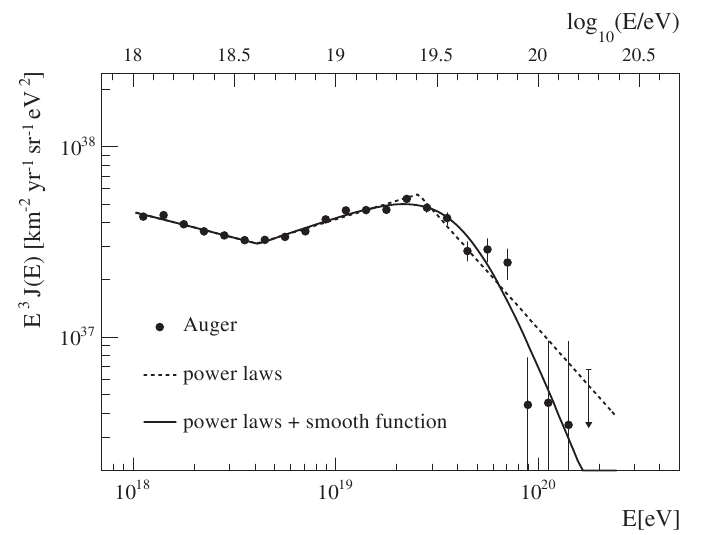
\includegraphics[width=0.75\textwidth]{fig/introduccion/spectrum_withGZK}
		\caption{\label{fig:specGZK} }
		\end{center}
	\end{figure}
	
	\section{Importancia de la detecci\'on de neutrinos c\'osmicos}

	VER EL PROPOSAL DE GRAND!
	
\begin{figure}[ht]
	\begin{center}
	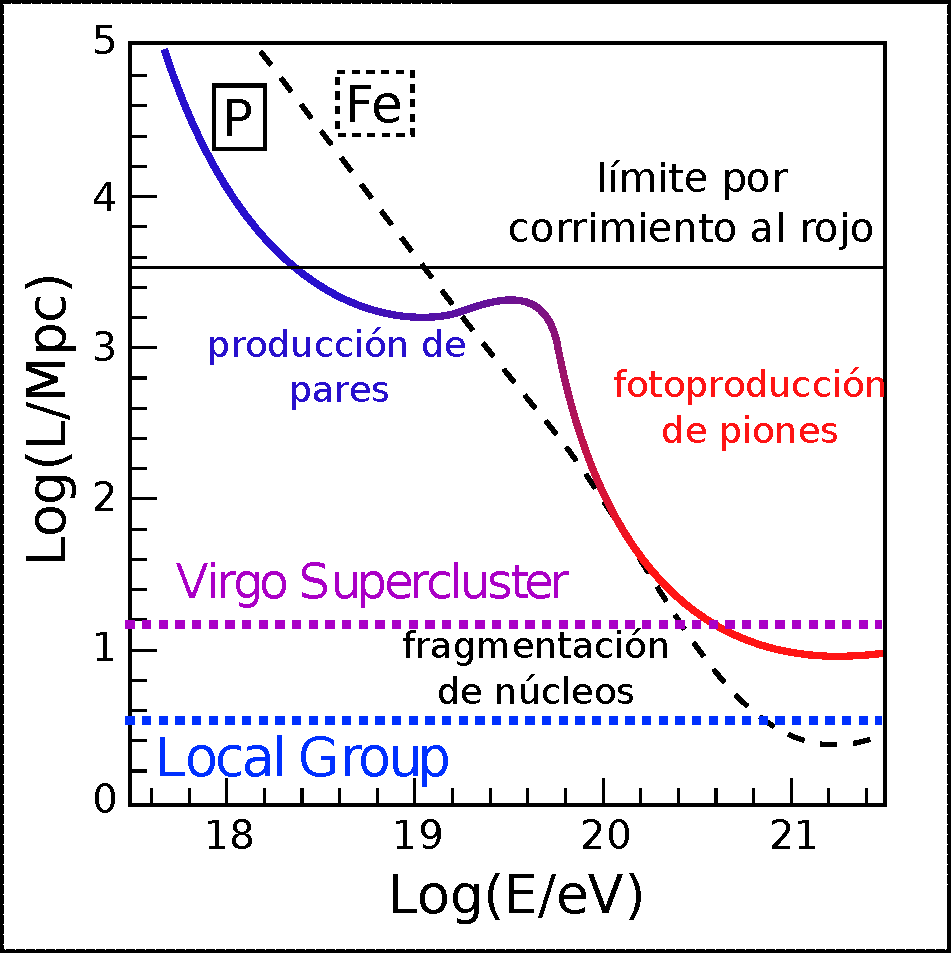
\includegraphics[width=0.75\textwidth]{fig/introduccion/proton_propaga_espanol}
	\caption{\label{fig:protProp} }
	\end{center}
\end{figure}


\begin{figure}[ht]
	\begin{center}
	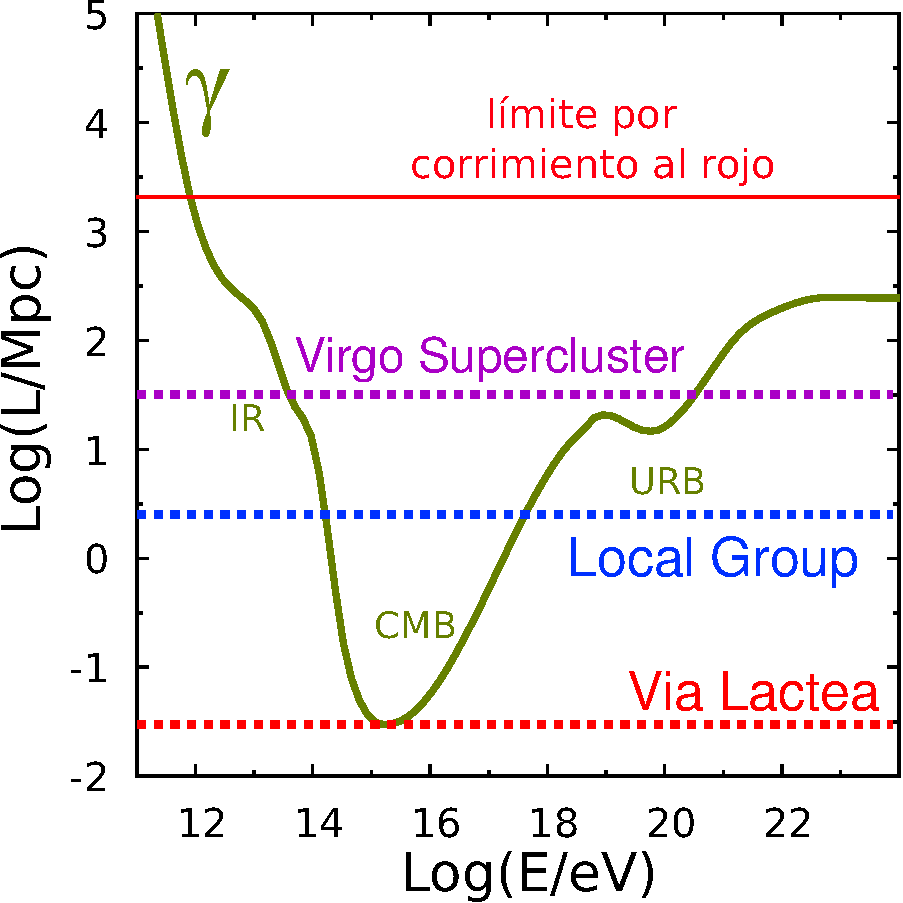
\includegraphics[width=0.75\textwidth]{fig/introduccion/photon_propaga_espanol}
	\caption{\label{fig:photProp} }
	\end{center}
\end{figure}

\section{Posibles fuentes y flujos esperados}

	\subsection{Neutrinos GZK}

	\begin{figure}[ht]
		\begin{center}
		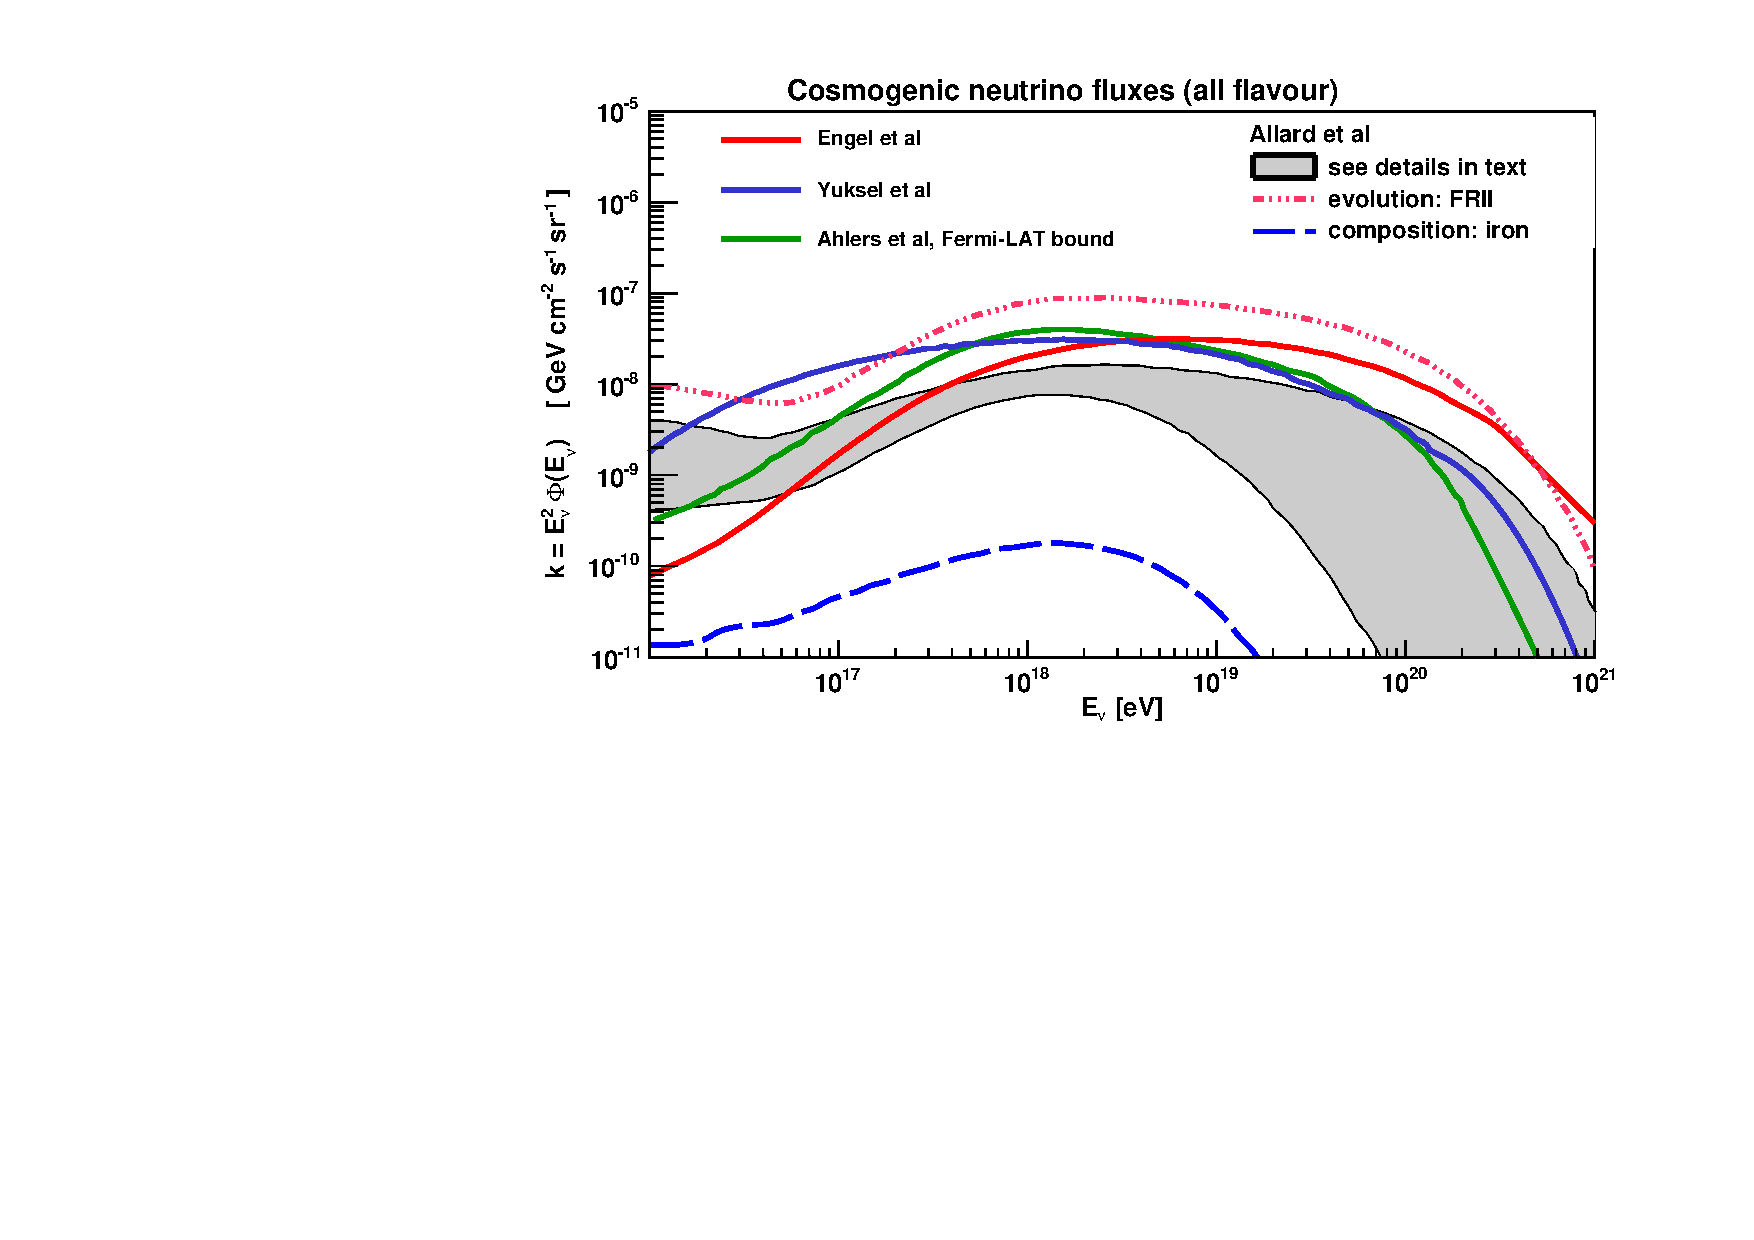
\includegraphics[width=\textwidth]{fig/introduccion/gzk_fluxes}
		\caption{\label{fig:flujosGZK} }
		\end{center}
	\end{figure}
	
	\subsection{AGNs y GRBs}
	
	\begin{figure}[ht]
		\begin{center}
		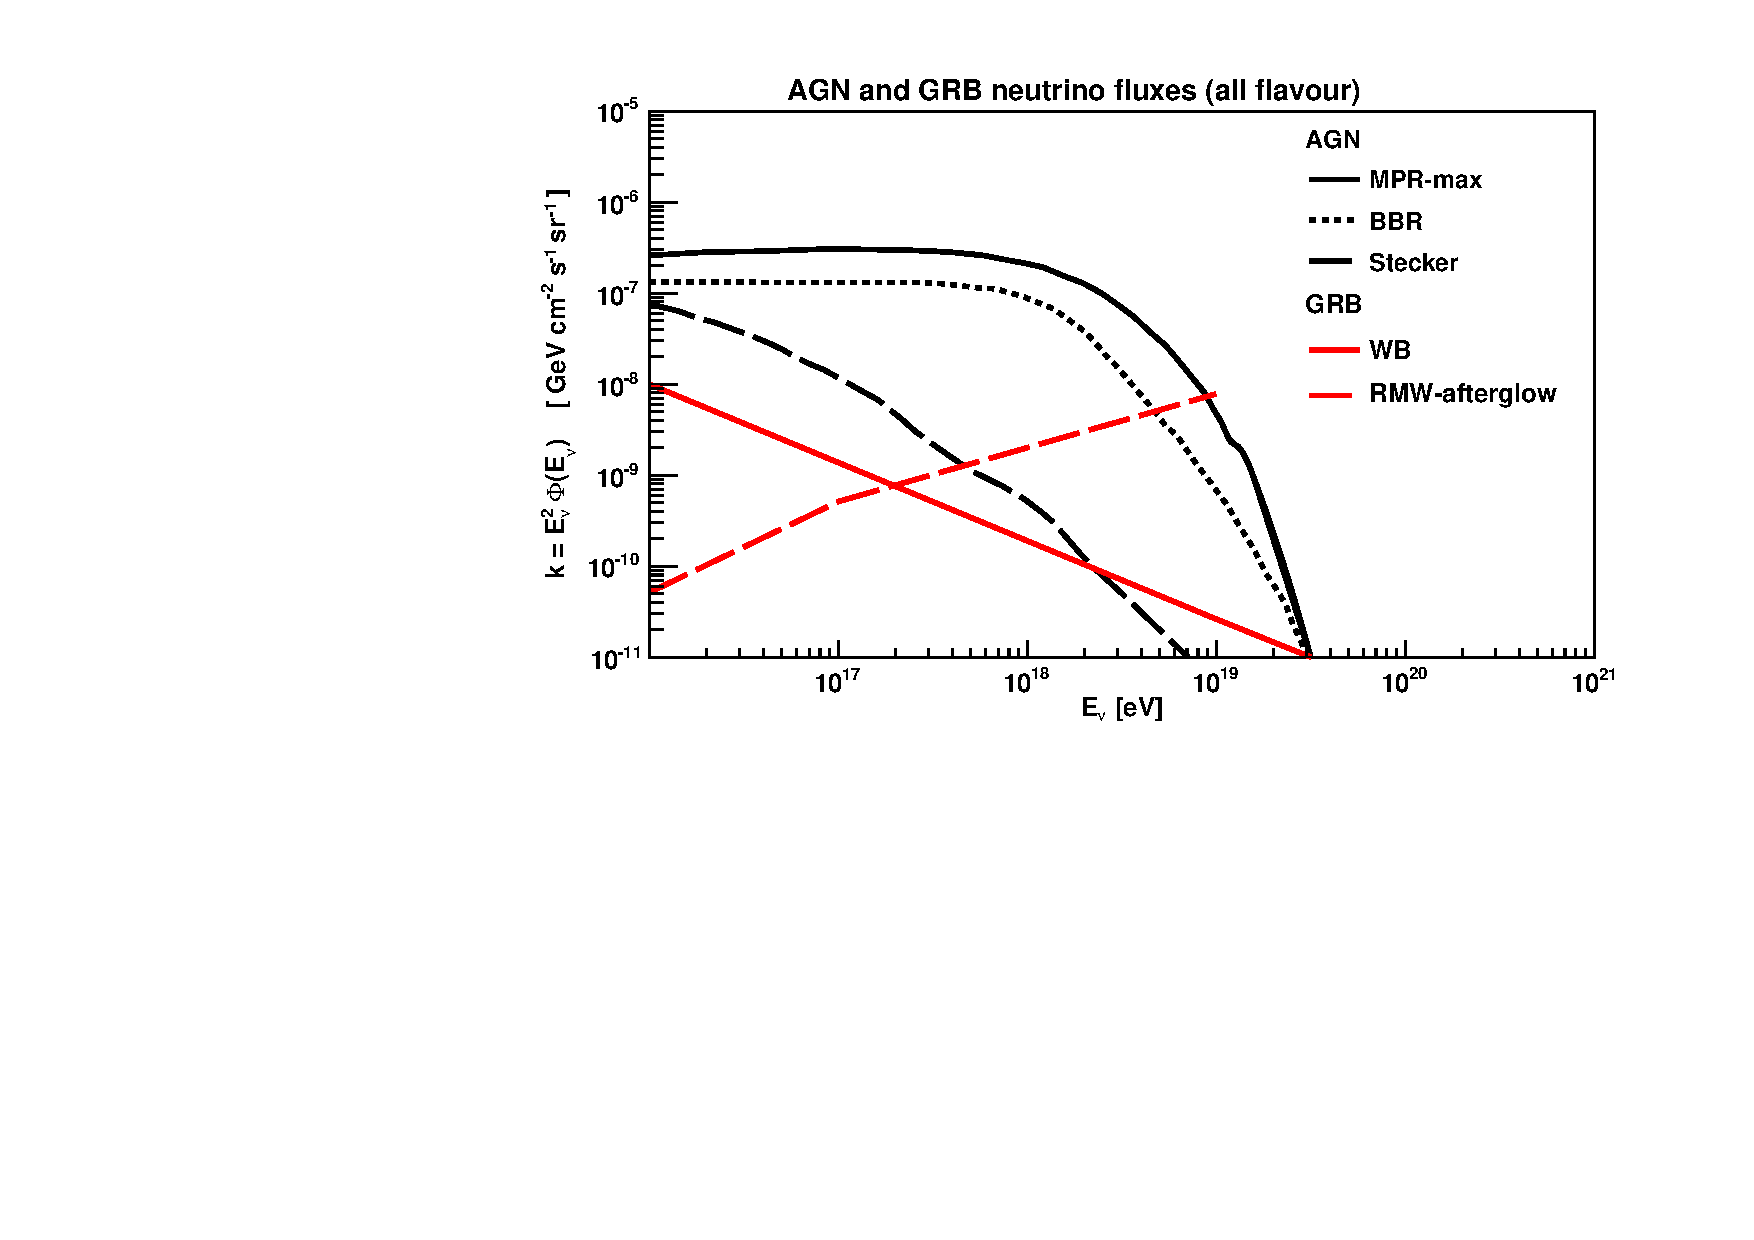
\includegraphics[width=0.75\textwidth]{fig/introduccion/AGN_GRB_nufluxes}
		\caption{\label{fig:flujosAGN} }
		\end{center}
	\end{figure}
	
	\subsection{Fuentes no convencionales}
	
	\begin{figure}[ht]
		\begin{center}
		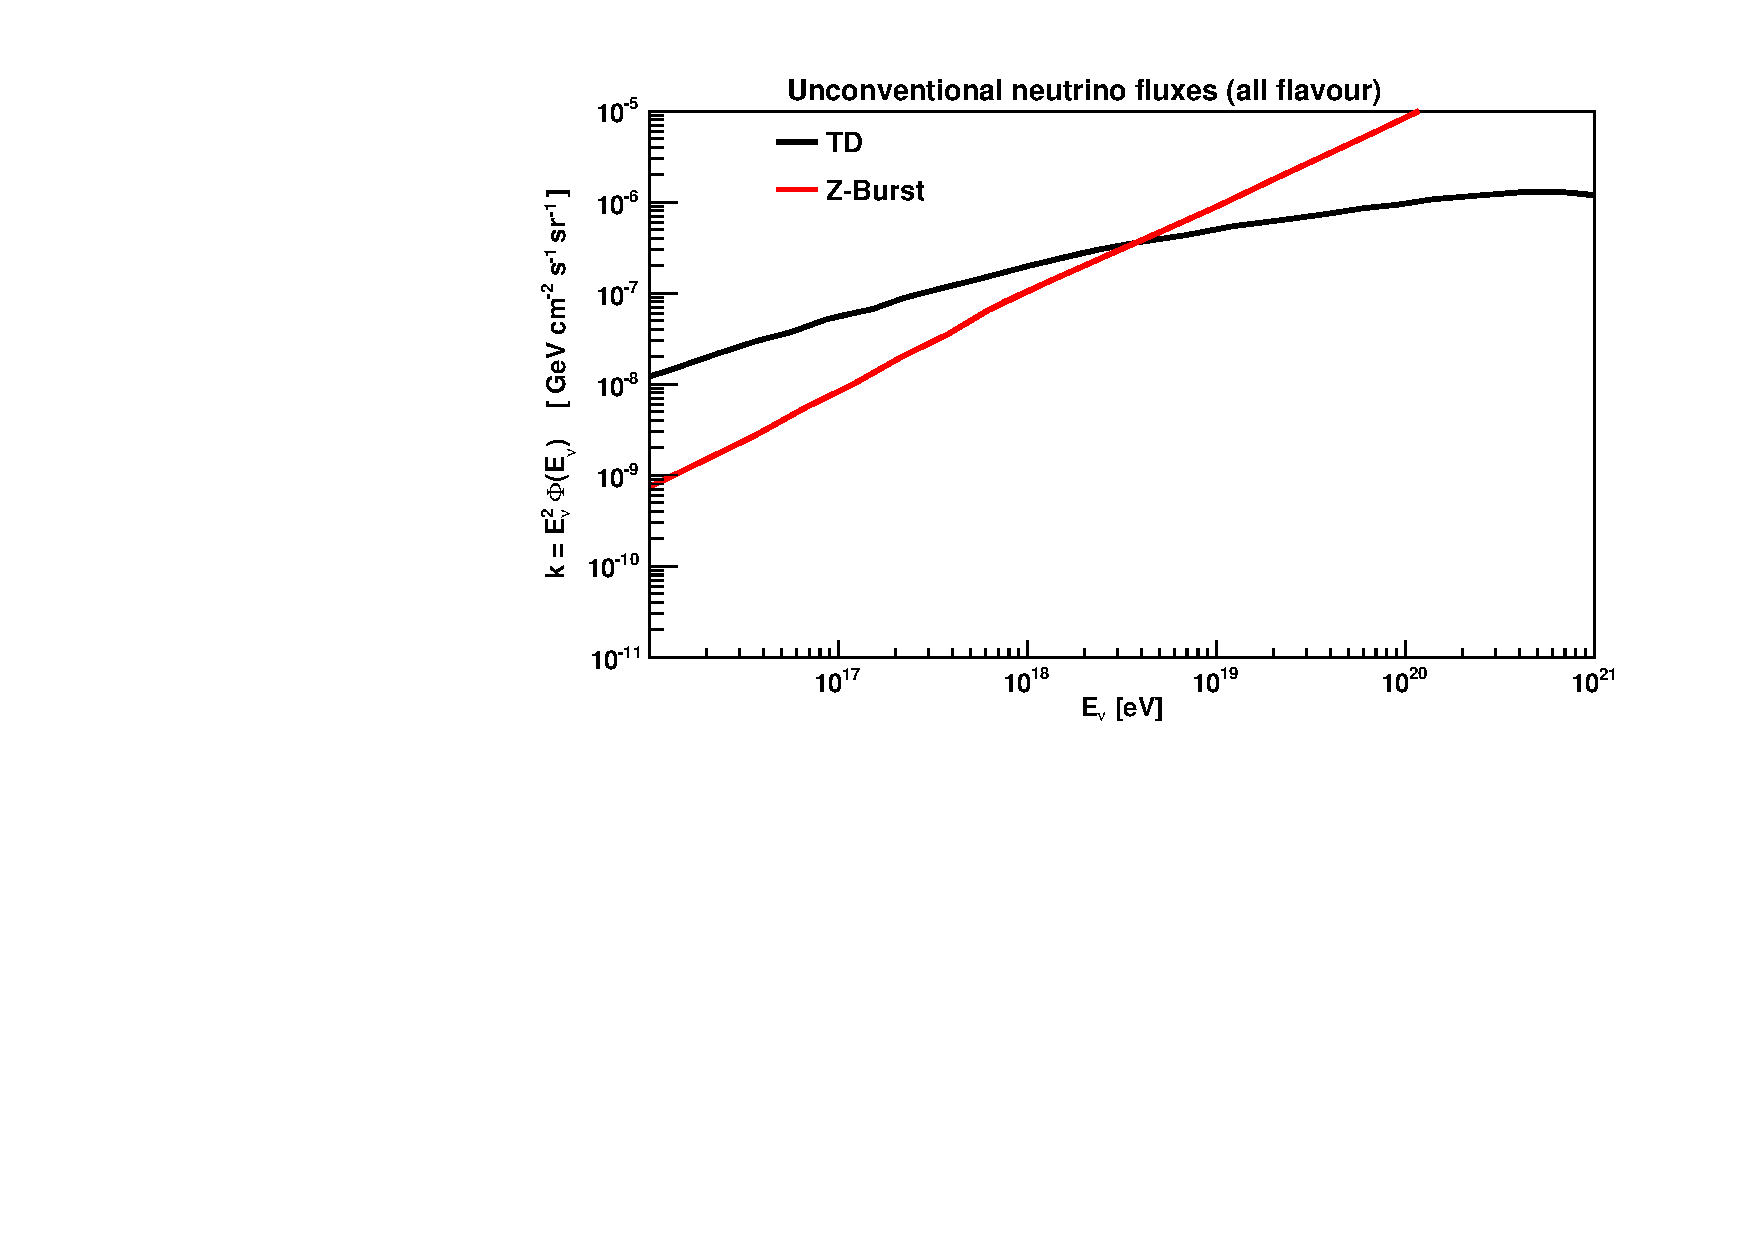
\includegraphics[width=0.75\textwidth]{fig/introduccion/unconventional_nuFluxes}
		\caption{\label{fig:flujosNoConv} }
		\end{center}
	\end{figure}

\section{Búsquedas de neutrinos cósmicos ultra energéticos}

\section{Nacimiento de la astronom\'ia de neutrinos c\'osmicos}

